In this section we provide an overview on how our system will look like.\\
A minimal part of the mockups had already been inserted in the RASD document, here we will illustrate them with an higher level of detail, focusing on the phone application.\\
We decided to do that because the web application and the phone application share the same functionalities, therefore it would have been redundant and not that useful to repeat the same concepts twice.
This also applies for the UX diagram.

\section{Mockups}
\label{subsect:Mockups}
	\begin{figure}[H]
		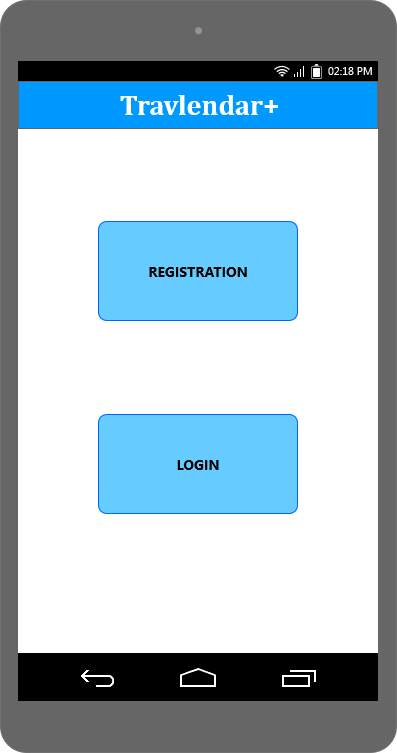
\includegraphics[scale=0.35]{mockup/app/Start/00-Start}
		\hspace{.3cm}
		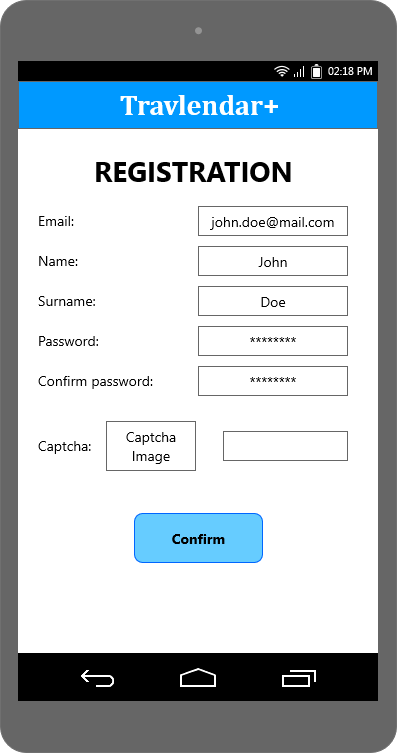
\includegraphics[scale=0.35]{mockup/app/Start/01-Register}
		\hspace{.3cm}
		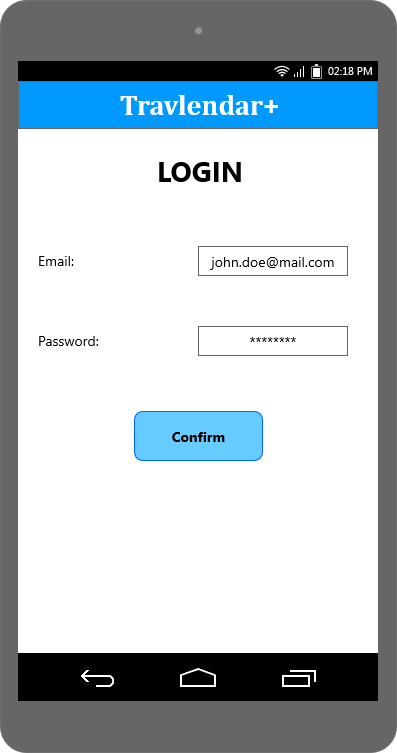
\includegraphics[scale=0.35]{mockup/app/Start/02-Login}
		\centering
		\caption{The user can register and log into the system.}
	\end{figure}
	
	\begin{figure}[H]
		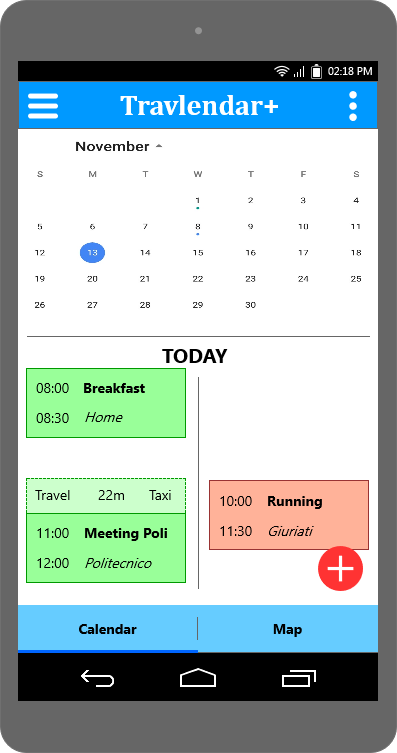
\includegraphics[scale=0.35]{mockup/app/Calendar/00-Calendar}
		\hspace{.3cm}
		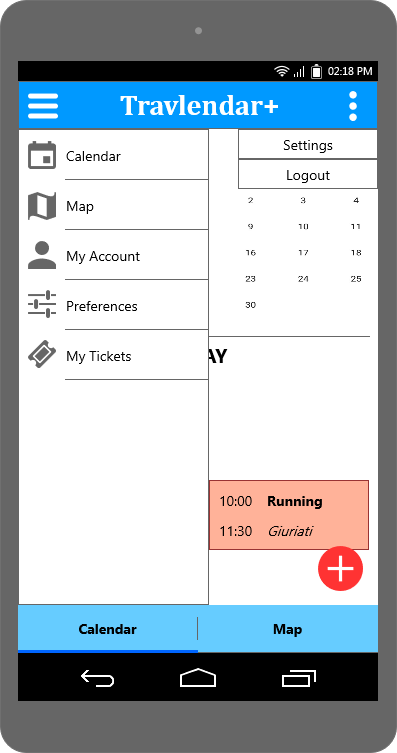
\includegraphics[scale=0.35]{mockup/app/03-Nav_Menu}
		\hspace{.3cm}
		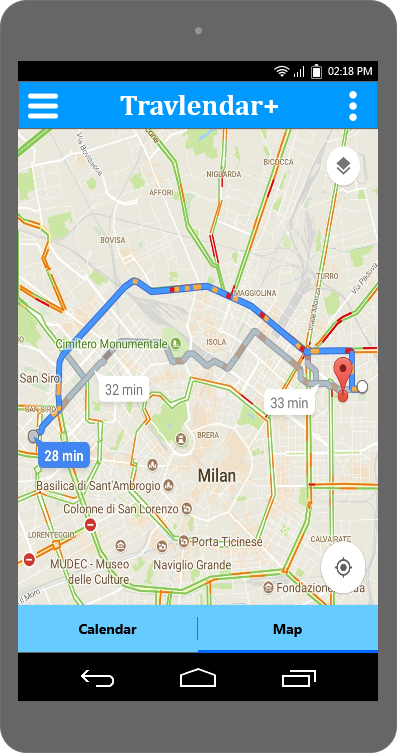
\includegraphics[scale=0.35]{mockup/app/04-Map}
		\centering
		\caption{The main screens of the application.}
	\end{figure}

	\begin{figure}[H]
		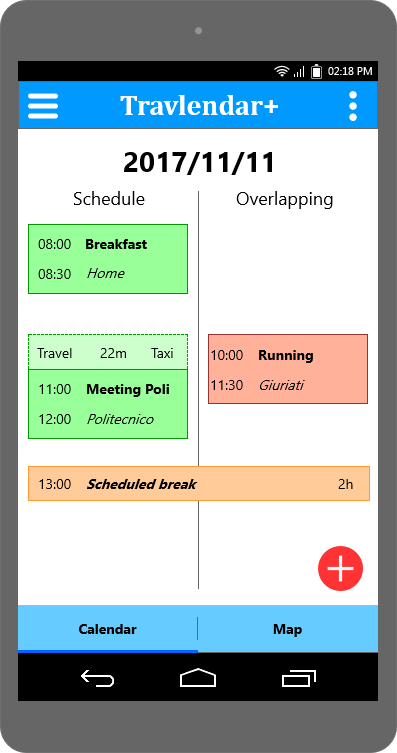
\includegraphics[scale=0.35]{mockup/app/Calendar/Schedule/00-Schedule}
		\hspace{.3cm}
		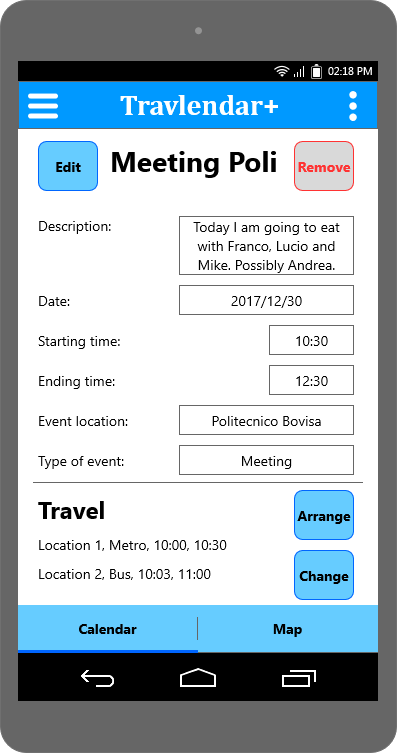
\includegraphics[scale=0.35]{mockup/app/Calendar/Schedule/01-View_Event}
		\centering 
		\caption{The user can see his schedule and view, edit or modify its events.}
	\end{figure}
	
	\begin{figure}[H]
		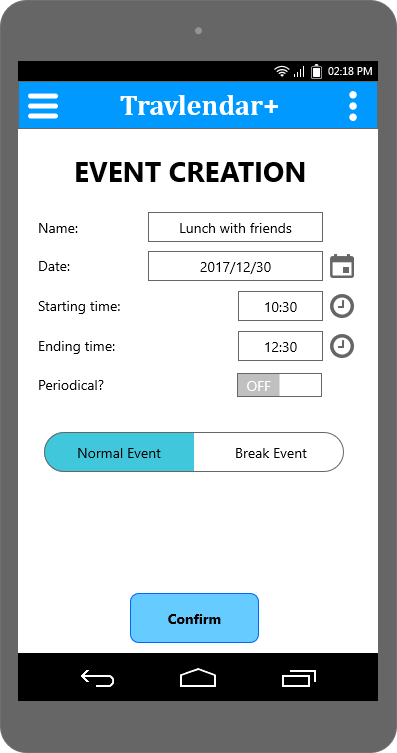
\includegraphics[scale=0.35]{mockup/app/Calendar/Create_Event/00-Create_Event}
		\hspace{.3cm}
		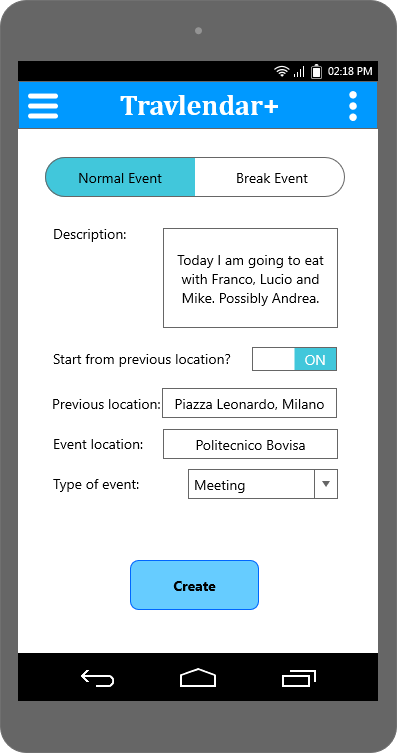
\includegraphics[scale=0.35]{mockup/app/Calendar/Create_Event/01-Create_Normal_Event}
		\hspace{.3cm}
		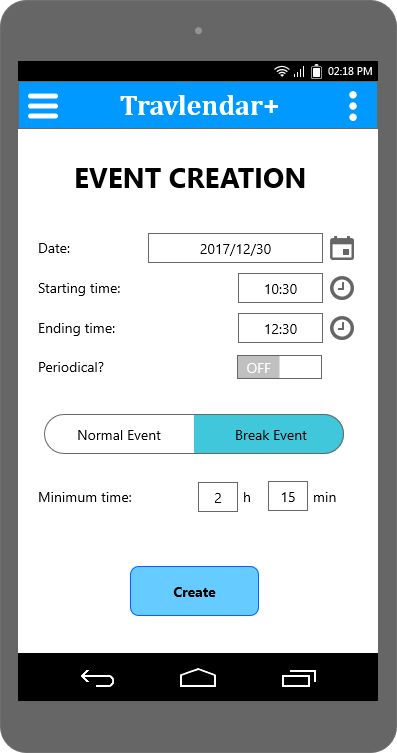
\includegraphics[scale=0.35]{mockup/app/Calendar/Create_Event/02-Create_Break_Event}
		\centering 
		\caption{The user can create an event, specifying if it's a break event or a normal one.}
	\end{figure}
	
	\begin{figure}[H]
		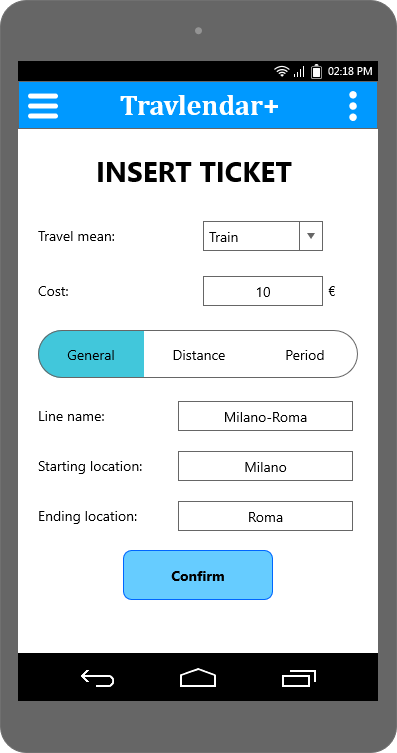
\includegraphics[scale=0.35]{mockup/app/My_Tickets/Add_Ticket/01-Add_General_Ticket}
		\hspace{.3cm}
		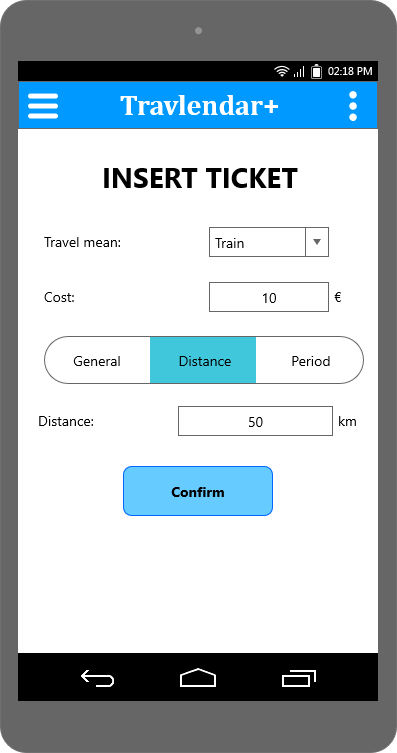
\includegraphics[scale=0.35]{mockup/app/My_Tickets/Add_Ticket/02-Add_Distance_Ticket}
		\hspace{.3cm}
		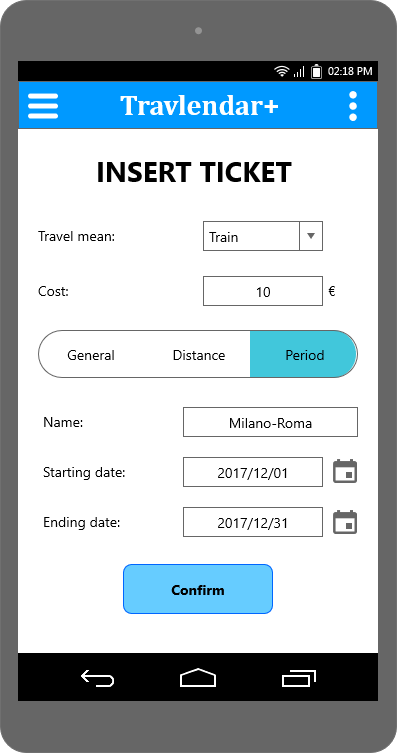
\includegraphics[scale=0.35]{mockup/app/My_Tickets/Add_Ticket/03-Add_Period_Ticket}
		\centering 
		\caption{The user can handle his tickets.}
	\end{figure}
	
	\begin{figure}[H]
		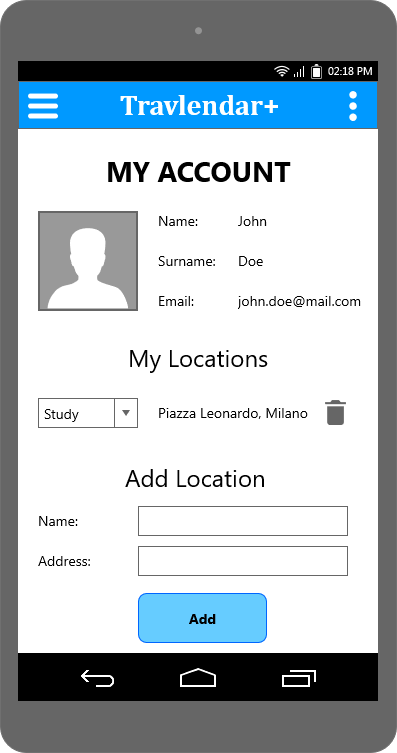
\includegraphics[scale=0.35]{mockup/app/05-My_Account}
		\hspace{.3cm}
		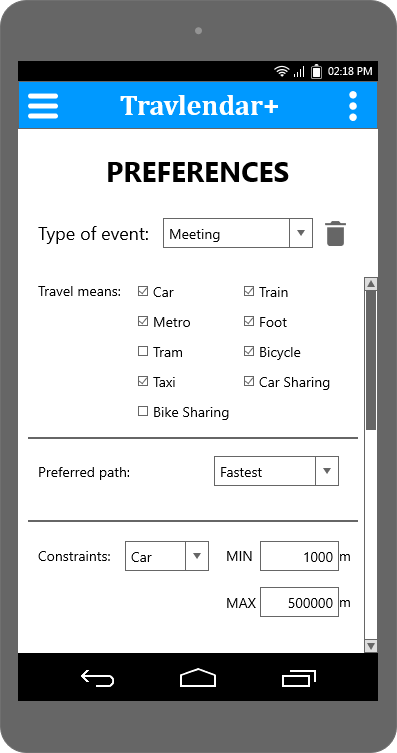
\includegraphics[scale=0.35]{mockup/app/06-Preferences}
		\hspace{.3cm}
		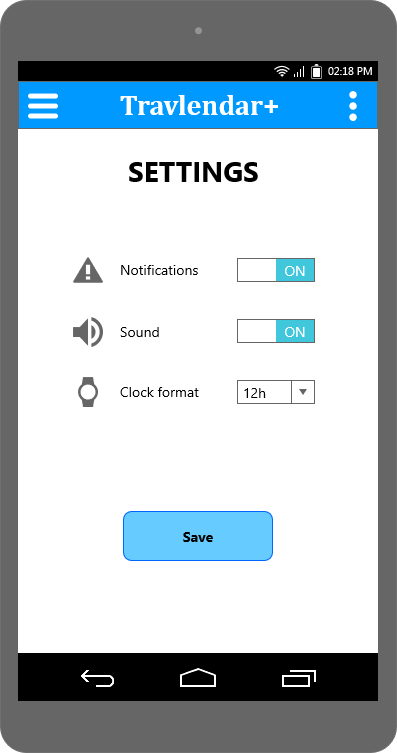
\includegraphics[scale=0.35]{mockup/app/08-Settings}
		\centering 
		\caption{The user can modify his preferences and the system settings.}
	\end{figure}

\section{UX diagrams}
\label{subsect:UX diagrams}

	\begin{figure}[H]
		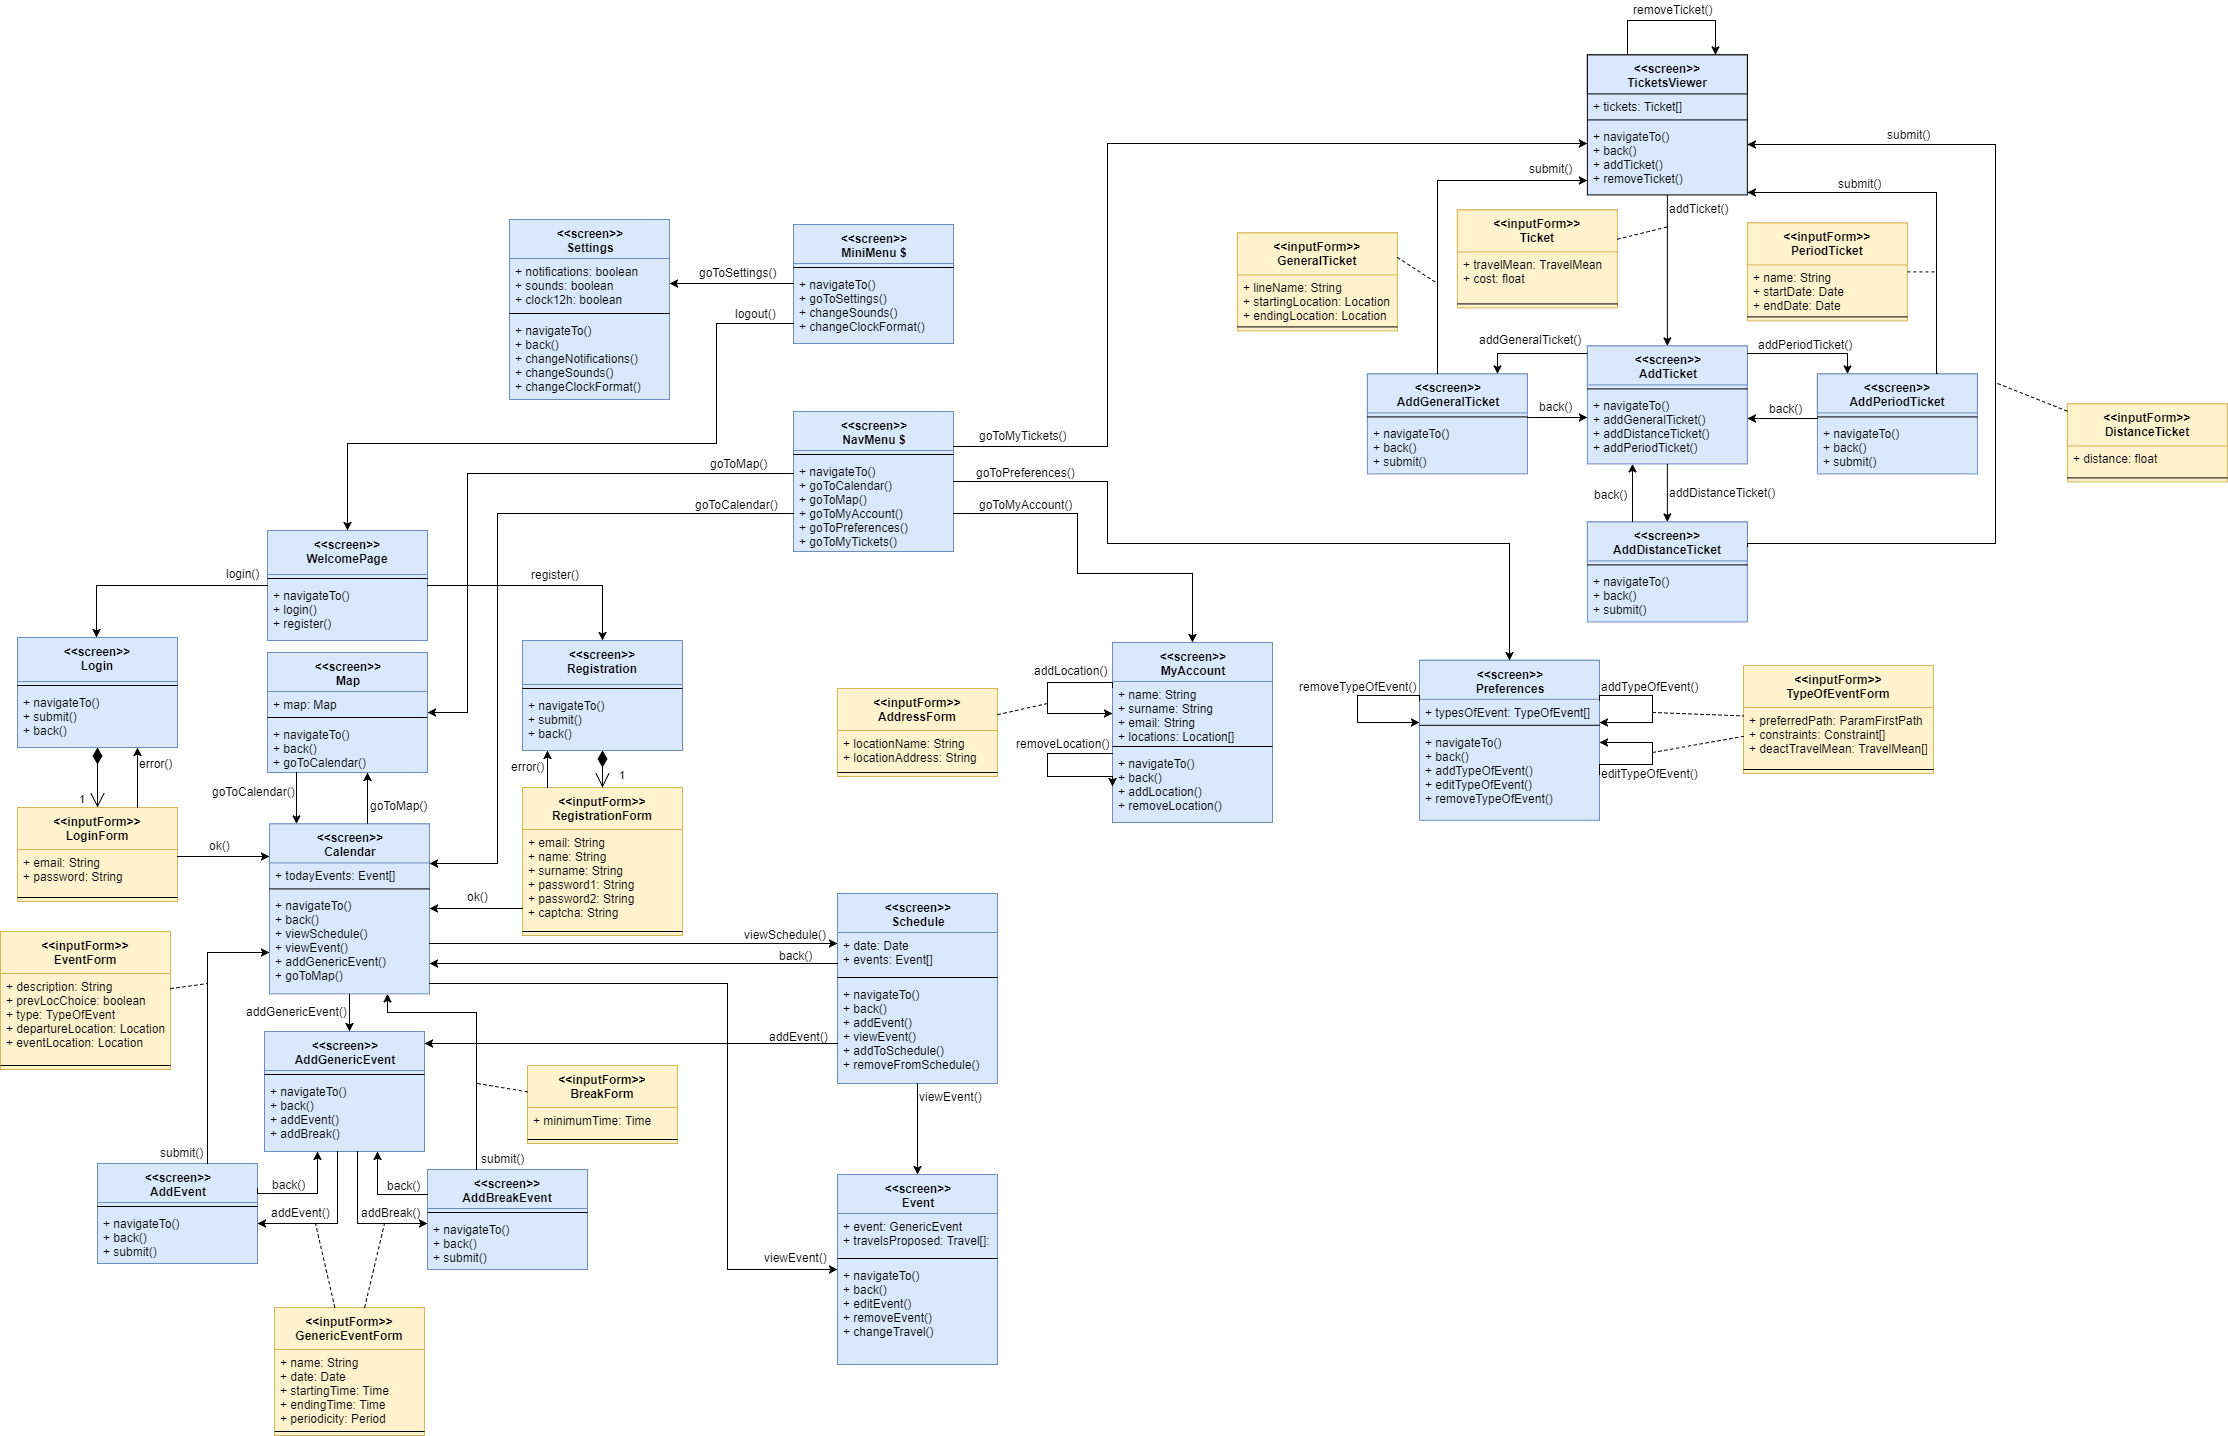
\includegraphics[width=\textheight, angle=90]{ux_diagram}
		\centering
	\end{figure}